\apendice{Documentación técnica de programación}

\section{Introducción}\label{introduccion}

En este anexo se describe la documentación técnica de programación,
incluyendo la instalación del entorno de desarrollo, la estructura de la
aplicación, su compilación, la configuración de los diferentes servicios
de integración utilizados o las baterías de test realizadas.

\section{Estructura de directorios}\label{estructura-de-directorios}

El repositorio del proyecto se distribuye de la siguiente manera:

\begin{itemize}
\tightlist
\item
  \texttt{/}: contiene los ficheros de configuración de Gradle, de los
  servicios de integración continua, el fichero README y la copia de la
  licencia.
\item
  \texttt{/app/}: módulo correspondiente a la aplicación.
\item
  \texttt{/app/src/}: código fuente de la aplicación.
\item
  \texttt{/app/src/main/}: contiene todas las clases comunes a todos los
  \emph{flavours}.
\item
  \texttt{/app/src/main/res/}: recursos de la aplicación
  (\emph{layouts}, menús, imágenes, cadenas de texto, etc.).
\item
  \texttt{/app/src/mock/}: \emph{mock flavour}, utilizado para inyectar
  componentes alternativos durante los test.
\item
  \texttt{/app/src/prod/}: \emph{prod flavour}, utilizado para inyectar
  los componentes que se utilizan en la versión de producción.
\item
  \texttt{/app/src/test/}: test unitarios.
\item
  \texttt{/app/src/testMock/}: test unitarios y de integración que
  necesitan inyectar componentes falsos.
\item
  \texttt{/app/src/androidTest/}: Android UI test.
\item
  \texttt{/docs/}: documentación del proyecto.
\item
  \texttt{/docs/img/}: imágenes utilizadas en la documentación.
\item
  \texttt{/docs/javadoc/}: documentación \emph{javadoc}.
\item
  \texttt{/docs/latex/}: documentación en formato \LaTeX.
\item
  \texttt{/docs/rst/}: documentación en formato reStructuredText.
\end{itemize}

Para saber más sobre la organización de un proyecto Android consultar
la documentación \citep{android:folders}.

\section{Manual del programador}\label{manual-del-programador-1}

El siguiente manual tiene como objetivo servir de referencia a futuros
programadores que trabajen en la aplicación. En él se explica cómo
montar el entorno de desarrollo, obtener el código fuente del proyecto,
compilarlo, ejecutarlo, testearlo y exportarlo.

\subsection{Entorno de desarrollo}\label{entorno-de-desarrollo}

Para trabajar con el proyecto se necesita tener instalados los
siguientes programas y dependencias:

\begin{itemize}
\tightlist
\item
  Java JDK 7.
\item
  Android Studio.
\item
  Git.
\item
  OpenCV.
\end{itemize}

A continuación, se indica como instalar y configurar correctamente cada
uno de ellos.

\subsubsection{Java JDK 7}\label{java-jdk-7}

El lenguaje de programación más popular para realizar aplicaciones
Android es Java. A día de hoy, Android no soporta la versión 8 de Java,
por lo que tenemos que trabajar con la versión 7. Podemos obtener esta
versión desde \citep{java:jdk7}. Se debe elegir correctamente el sistema
operativo y la arquitectura del ordenador y, posteriormente, seguir el
asistente de instalación.

\subsubsection{Android Studio}\label{android-studio}

Android Studio es el IDE oficial para el desarrollo de aplicaciones
Android. Está basado en IntelliJ IDEA de JetBrains. Proporciona soporte
para Gradle, emulador, editor de \emph{layouts}, refactorizaciones
específicas de Android, herramientas Lint para detectar problemas de
rendimiento, uso, compatibilidad de versión, etc.

Se puede obtener desde \citep{android:androidstudio}. Junto con Android
Studio se instala también el Android SDK y \emph{Android Virtual Device}
(AVD).

\imagen{android-studio}{Android Studio.}

\subsubsection{Git}\label{git}

Para hacer uso del repositorio se necesita tener instalado el gestor de
versiones Git. Este programa nos permitirá clonar el repositorio,
movernos por sus diferentes ramas, etiquetas, etc. Se puede obtener
desde \citep{git:scm}. Una vez instalado, trabajaremos con Git
Bash.

\imagen{git-clone}{Terminal Git Bash.}

\subsubsection{OpenCv}\label{opencv}

OpenCV es un paquete \emph{Open Source} de visión artificial que
contiene más de 2500 librerías de procesamiento de imágenes y visión
artificial, escritas en C/C\texttt{++} a bajo/medio nivel.

Para ejecutar OpenCV en un dispositivo Android se necesita tener
instalado la aplicación
\href{https://play.google.com/store/apps/details?id=org.opencv.engine}{OpenCV
Manager}. Sin embargo, para el desarrollo de la aplicación también
debemos instalar la versión de escritorio de OpenCV para poder ejecutar
los test de integración del algoritmo en local.

Podemos obtener OpenCV desde la página oficial \citep{opencv:web}. En
este proyecto hemos utilizado la versión 3.2.

Una vez instalada, tenemos que añadir al \emph{path} de Windows el
directorio donde se encuentran los ejecutables
(\texttt{opencv/build/java/x64} o \texttt{x86}).

\imagen{opencv-var}{Variable del sistema de OpenCV.}

En la página web oficial se puede obtener información más detallada
sobre el proceso de instalación.

\subsection{Obtención del código
fuente}\label{obtencion-del-codigo-fuente}

Para el desarrollo de la aplicación se ha utilizado un repositorio Git
hospedado en GitHub. Para obtener una copia de este hay que proceder de
la siguiente manera:

\begin{enumerate}
\def\labelenumi{\arabic{enumi}.}
\tightlist
\item
  Abrir la terminal Git Bash.
\item
  Desplazarse al directorio donde se desee copiar el repositorio
  (utilizando el comando \texttt{cd}).
\item
  Introducir el siguiente comando:\\
  \texttt{git\ clone\ https://github.com/davidmigloz/go-bees.git}
\item
  Se iniciará la descarga del repositorio, cuando finalice se dispondrá
  de una copia completa de este.
\end{enumerate}

\begin{figure}[H]
	\centering
	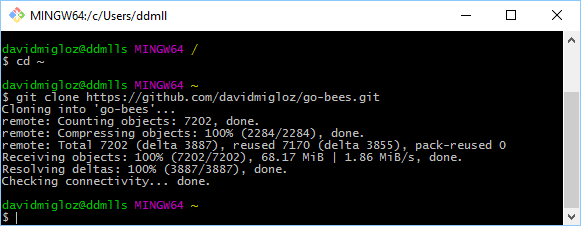
\includegraphics[width=0.9\textwidth]{git-clone}
	\caption{Clonar repositorio de GitHub.}\label{fig:git-clone-1}
\end{figure}

Para conocer el proceso detalladamente consultar \citep{github:clone}.

\subsection{Importar proyecto en Android
Studio}\label{importar-proyecto-en-android-studio}

Una vez obtenido el código fuente de la aplicación, tenemos que
importarlo como proyecto de Android Studio. Para ello, hay que seguir
los siguientes pasos:

\begin{enumerate}
\def\labelenumi{\arabic{enumi}.}
\tightlist
\item
  Abrir Android Studio.
\item
  Menú \texttt{File\ \textgreater{}\ Open\ldots{}}
\item
  Buscamos el directorio donde hemos clonado el repositorio.
\item
  Dentro del repositorio, seleccionamos el archivo
  \texttt{build.gradle}.
\item
  Android Studio detectará que es un proyecto Android y lo importará
  automáticamente.
\item
  Si alguna característica de las que hace uso la aplicación no se
  encuentra instalada, Android Studio mostrará un mensaje de error con
  un enlace para instalar la característica en cuestión.
\end{enumerate}

\begin{figure}[H]
	\centering
	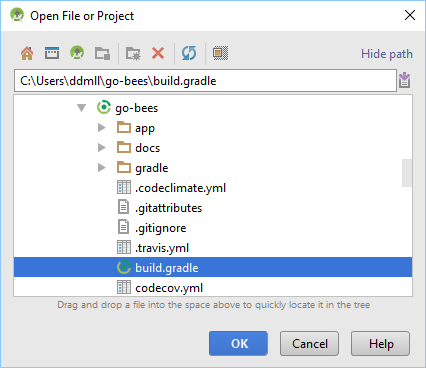
\includegraphics[width=0.4\textwidth]{android-studio-import}
	\caption{Importar proyecto en Android Studio.}\label{fig:android-studio-import}
\end{figure}

Para conocer el proceso detalladamente consultar \citep{android:import}.

\subsection{Añadir nuevas características a la
aplicación}\label{anadir-nuevas-caracteristicas-a-la-aplicacion}

Tras importar el proyecto en Android Studio, ya estamos en disposición
de realizar modificaciones de la aplicación.

Para añadir una nueva característica siguiendo la arquitectura MVP, la
convención de paquete por característica y las metodologías TDD y
GitFlow, se deben seguir los siguientes pasos generales.

\begin{enumerate}
\def\labelenumi{\arabic{enumi}.}
\tightlist
\item
  Crear una nueva rama (\emph{feature branch}) desde la rama
  \emph{develop}:\\
  \texttt{git\ checkout\ -b\ export-data\ develop}
\item
  Crear un nuevo paquete con el nombre de la característica que se desea
  añadir (ej. \texttt{exportdata}).
\item
  Crear una interfaz (ej. \texttt{ExportDataContract.java}) que contenga
  a su vez dos interfaces. En una se deben definir las responsabilidades
  del \emph{presenter} y en la otra las de la vista. Hacer
  \emph{commit}: \\ 
  \texttt{git\ add\ -A} \\
  \texttt{git\ commit\ -m\ "Add\ export\ data\ contract\ \#x"}
\item
  Crear una clase para el \emph{presenter} (ej.\\
  \texttt{ExportDataPresenter.java}) que implemente su correspondiente
  interfaz anterior (no añadir ninguna lógica todavía). Hacer
  \emph{commit}.
\item
  Crear una clase para la vista (ej. \texttt{ExportDataFragment}) que
  descienda de \texttt{Fragment} e implemente su correspondiente
  interfaz anterior (no añadir ninguna lógica todavía). Hacer
  \emph{commit}.
\item
  Crear una clase que descienda de \texttt{AppCompatActivity} (ej. \\
  \texttt{ExportDataActivity.java}) y que enlace el modelo, el
  \emph{presenter} y la vista. Hacer \emph{commit}.
\item
  Crear un test sobre el \emph{presenter} de acuerdo a los requisitos.
  Hacer \emph{commit}.
\item
  Ejecutar el test y comprobar que no pasa.
\item
  Implementar las clases anteriores hasta conseguir que pasen el test.
  Hacer \emph{commit}.
\item
  Refactorizar el código para mejorar su calidad. Hacer \emph{commit}.
\item
  Añadir un \emph{intent} desde donde se quiera acceder a esa
  característica. Hacer \emph{commit}.
\item
  Una vez que se ha implementado correctamente la característica, se
  debe incorporar a la rama \emph{develop} y sincronizar con GitHub:\\
  \texttt{git\ checkout\ develop}\\
  \texttt{git\ merge\ -\/-no-ff\ export-data}\\
  \texttt{git\ branch\ -d\ myfeature}\\
  \texttt{git\ push\ origin\ develop}
\end{enumerate}

\subsection{Actualizar dependencias}\label{actualizar-dependencias}

Una tarea de mantenimiento común es la actualización de las dependencias
de la aplicación. Es importante tenerlas actualizadas para evitar
problemas de seguridad o funcionalidad que pudiesen tener en versiones
anteriores.

El proyecto utiliza Gradle como sistemas de construcción automática del
\emph{software}. Una de sus funcionalidades es la gestión de
dependencias. Esta permite al desarrollador definir las dependencias de
su aplicación, sus versiones y los repositorios donde se hospedan y
Gradle se encarga de descargarlas e importarlas al proyecto
automáticamente.

Las dependencias se definen en el fichero \texttt{build.gradle} del
módulo de la aplicación (\texttt{go-bees/app/build.gradle}):

\begin{figure}[H]
	\centering
	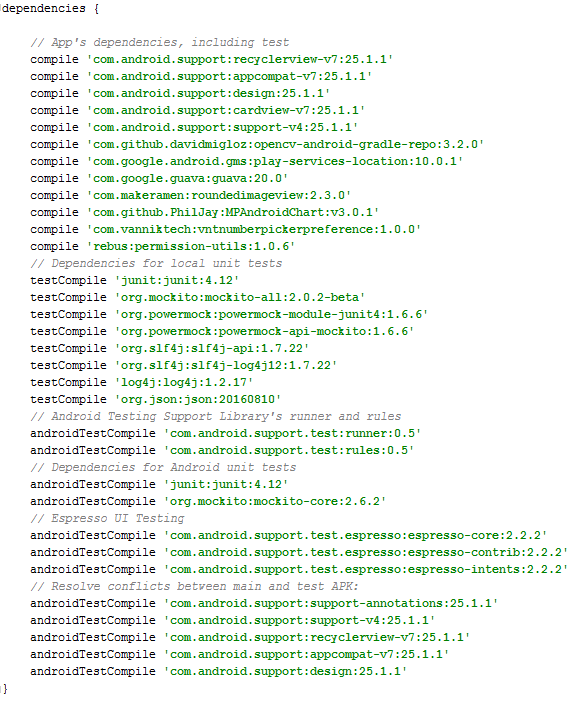
\includegraphics[width=0.8\textwidth]{dependences}
	\caption{Dependencias del proyecto.}\label{fig:dependences}
\end{figure}

Se puede observar que existen tres formas de importar las dependencias,
cada una define con un ámbito de aplicación distinto:

\begin{itemize}
\tightlist
\item
  \texttt{Compile}: estará disponible para el código de la aplicación.
\item
  \texttt{testCompile}: estará disponible en los test unitarios de la
  aplicación.
\item
  \texttt{androidTestCompile}: estará disponible en los test de
  instrumentación de la aplicación.
\end{itemize}

Para actualizar la versión de una dependencia, solamente hay que
actualizar el número de la versión que figura en la importación.
Posteriormente, se debe sincronizar Gradle (\emph{Sync Project with
Gradle Files}).

\subsection{Compilar código fuente}\label{compilar-codigo-fuente}

La compilación del proyecto se realiza mediante la tarea \texttt{build}
de Gradle. Podemos ejecutarla por línea de comandos
(\texttt{./gradlew\ build}) o mediante la interfaz de Android Studio.

\begin{figure}[H]
	\centering
	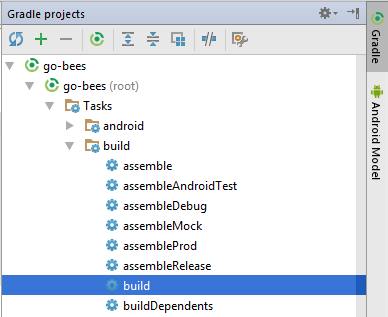
\includegraphics[width=0.5\textwidth]{gradle-build}
	\caption{Compilar proyecto.}\label{fig:gradle-build}
\end{figure}

Todos los ficheros generados durante la compilación se guardan en la
carpeta \texttt{build} del proyecto.

Para conocer el proceso detalladamente consultar
\citep{android:compilerun}.

\subsection{Ejecutar aplicación}\label{ejecutar-aplicacion}

La aplicación se puede ejecutar en un dispositivo real o en un emulador.

\subsubsection{Dispositivo real}\label{dispositivo-real}

Para ejecutar la aplicación en un dispositivo real, se debe conectar
este al equipo de desarrollo mediante un cable USB. El equipo debe tener
los \emph{drivers} del dispositivo instalado, sino no lo reconocerá.

Una vez conectado el dispositivo:

\begin{enumerate}
\def\labelenumi{\arabic{enumi}.}
\tightlist
\item
  Presionar el botón \emph{Run}.
\item
  Si el equipo reconoce el dispositivo se mostrará su nombre debajo de
  ``\emph{Connected Devices}''.
\item
  Seleccionar el dispositivo y pulsa \emph{Ok}.
\item
  Se transferirá el ejecutable de la aplicación y se instalará.
\item
  Una vez instalada, se podrá utilizar la aplicación desde el
  dispositivo.
\end{enumerate}

\subsubsection{Emulador}\label{emulador}

Un emulador (denominados \emph{Android Virtual Device} - AVD) es una
aplicación que simula el funcionamiento de un dispositivo real Android.
La creación y gestión de los emuladores se hace a través de \emph{AVD
Manager}.

Para ejecutar la aplicación en un emulador:

\begin{enumerate}
\def\labelenumi{\arabic{enumi}.}
\tightlist
\item
  Presionar el botón de Run.
\item
  Si ya se posee algún emulador instalado, se mostrará en la lista de
  \emph{Android Virtual Devices}.
\item
  Si no, presionar el botón ``\emph{Create New Virtual Device}''.
\item
  Seleccionar las características que se deseen para el emulador y pulsa
  finalizar.
\item
  Seleccionar el emulador creado y pulsar \emph{Ok}.
\item
  Se iniciará el emulador y se instalará la aplicación en él.
\item
  Una vez instalada, se podrá utilizar la aplicación desde el emulador.
\end{enumerate}

Para conocer el proceso detalladamente consultar
\citep{android:compilerun}.

\subsection{Exportar aplicación}\label{exportar-aplicaciuxf3n}

Para exportar la aplicación como un fichero \texttt{.apk}:

\begin{enumerate}
\def\labelenumi{\arabic{enumi}.}
\tightlist
\item
  Menú \emph{Build} \textgreater{} \emph{Generate APK}.
\item
  Se generará un archivo \texttt{apk} y se guardará en
  \texttt{build/output/apk}.
\end{enumerate}

Si el \texttt{apk} que se desea generar es para distribuirlo en Google
Play, este debe estar firmado. Para ello:

\begin{enumerate}
\def\labelenumi{\arabic{enumi}.}
\tightlist
\item
  Menú \emph{Build} \textgreater{} \emph{Generate Signed APK}.
\item
  Se debe seleccionar el archivo \texttt{.jks} con la clave e introducir
  su contraseña. Si no se dispone de una clave, se puede generar
  siguiendo el asistente.
\item
  Se generará un archivo \texttt{apk} firmado apto para subir al Google
  Play.
\end{enumerate}

Para conocer el proceso detalladamente consultar
\citep{android:compilerun}.

\subsection{Servicios de integración
continua}\label{servicios-de-integracion-continua}

En el repositorio se han integrado varios servicios de integración
continua para detectar fallos en el software lo antes posible,
reduciendo el impacto de estos y aumentando la calidad del código.

A continuación, se describe cada servicio y se indica cómo configurarlo.

\subsubsection{TravisCI}\label{travisci}

TravisCI es una plataforma de integración continua en la nube para
proyectos alojados en GitHub. Permite realizar una \emph{build} del
proyecto y testearla automáticamente cada vez que se realiza un
\emph{commit}, devolviendo un informe con los resultados.

Para integrar Travis en el repositorio hospedado en GitHub se debe crear
una cuenta en su página web y dar permisos de acceso al repositorio. Una
vez asociado el servicio, este se configura mediante el fichero
\texttt{travis.yml}.

Las secciones más importantes de este fichero son:

\begin{itemize}
\tightlist
\item
  \texttt{sudo}: permite definir si el usuario de la máquina virtual
  tendrá privilegios o no.
\item
  \texttt{language}: permite definir el lenguaje de programación del
  proyecto.
\item
  \texttt{jdk}: permite definir la versión del JDK.
\item
  \texttt{compiler}: permite definir el compilador.
\item
  \texttt{addons}: permite configurar \emph{plugins} instalados en
  Travis (como, por ejemplo, el \emph{plugin} de SonarQube).
\item
  \texttt{env}: permite definir variables de entorno.
\item
  \texttt{android}: permite definir las dependencias Android del
  proyecto.
\item
  \texttt{licenses}: permite aceptar las licencias de las dependencias.
\item
  \texttt{before\_install}: en esta sección se pueden definir comandos a
  ejecutar antes de los comandos de la sección \texttt{install} (por ejemplo,
  actualizar la lista de paquetes).
\item
  \texttt{install}: en esta sección se deben definir aquellos comandos
  que instalen alguna dependencia (en nuestro caso
  \texttt{python-numpy}, necesaria para compilar OpenCV).
\item
  \texttt{before\_script}: en esta sección se pueden definir comandos a
  ejecutar antes de la sección script. En nuestro caso, nos descargamos
  el código fuente de OpenCV y lo compilamos.
\item
  \texttt{script}: en esta sección se realiza la compilación del
  proyecto y se ejecutan los diferentes test unitarios y de integración.
  Además, lanza un emulador y ejecuta los test de interfaz. También
  ejecuta el motor de chequeo de SonarQube.
\item
  \texttt{after\_success}: esta sección se utiliza para recolectar datos
  generados en las secciones anteriores. En nuestro caso, se envían los
  diferentes informes de ejecución de los test a el servicio Codecov.
\item
  \texttt{cache}: permite definir los directorios a cachear entre
  ejecuciones.
\end{itemize}

Los \emph{log} de ejecución de Travis son accesibles desde
\citep{travis:gobees}.

\imagen{travis}{TravisCI.}

Para saber más, acceder a su documentación \citep{travis:doc}.

\subsubsection{Codecov}\label{codecov}

Codecov es una herramienta que permite medir el porcentaje de código que
está cubierto por un test. Además, realiza representaciones visuales de
la cobertura y gráficos de su evolución.

La forma de integrarlo en el repositorio es idéntica a cómo se hizo con
Travis. Adicionalmente, hay que configurar el \emph{script} que ejecuta
Travis para que al finalizar su ejecución envíe los resultados a
Codecov.

\texttt{after\_success:\ \ bash\ \textless{}(curl\ -s\ https://codecov.io/bash)}

La configuración de Codecov se define en el archivo
\texttt{codecov.yml}.

\imagen{codecov}{Codecov.}

Para saber más, acceder a su documentación \citep{codecov:doc}.

\subsubsection{CodeClimate}\label{codeclimate}

Codeclimate es una herramienta que realiza revisiones de código
automáticamente.

La integración se realiza de forma similar a Travis. Su fichero de
configuración es \texttt{.codeclimate.yml}.

En nuestro proyecto hemos activado los siguientes motores de chequeo:
\emph{checkstyle}, \emph{fixme}, \emph{markdownlint} y \emph{pmd}.

CodeClimate utiliza el sistema de puntación GPA (\emph{Grade Point
Average}) para indicar el rendimiento general del proyecto. La nota
máxima se corresponde con un 4.0.

Los resultados de los chequeos se encuentran disponibles en
\citep{codeclimate:gobees}.

\imagen{codeclimate}{CodeClimate.}

Para saber más, acceder a su documentación \citep{codeclimate:doc}.

SonarQube es una plataforma de código abierto para la revisión continua
de la calidad de código. Permite detectar código duplicado, violaciones
de estándares, cobertura de test unitarios, \emph{bugs} potenciales,
etc.

Para integrar el servicio hay que seguir los siguientes pasos:

\begin{enumerate}
\def\labelenumi{\arabic{enumi}.}
\tightlist
\item
  Crear una cuenta en
  \href{http://www.sonarqube.com}{www.sonarqube.com}.
\item
  Generar un \emph{token} de autenticación.
\item
  Instalar el plugin de SonarQube para Gradle (\texttt{org.sonarqube}).
\item
  Configurar SonarQube en el fichero de configuración de Gradle
  (\texttt{build.gradle}).
\item
  Ejecutar la nueva tarea sonarqube de Gradle desde Travis.
\end{enumerate}

\imagen{sonarqube-config}{Configuración de SonarQube en Gradle.}

Los resultados de los análisis son accesibles desde
\citep{sonarqube:gobees}.

\imagen{sonarqube}{SonarQube.}

Para saber más, acceder a su documentación \citep{sonarqube:doc}.

\subsubsection{VersionEye}\label{versioneye}

VersionEye es una herramienta que monitoriza las dependencias del
proyecto y envía notificaciones cuando alguna de estas está
desactualizada, es vulnerable o viola la licencia del proyecto.

El servicio se integra de forma similar a Travis. No necesita fichero de
configuración.

Cuando se libera una nueva versión de alguna dependencia o se publica
alguna vulnerabilidad, VersionEye manda una notificación. Se puede
acceder a los informes desde \citep{versioneye:gobees}.

\imagen{versioneye}{VersionEye.}

Para saber más, acceder a su documentación \citep{versioneye:doc}.

\subsubsection{Read the Docs}\label{read-the-docs}

Read the Docs es un servicio de documentación continua que permite crear
y hospedar una página web generada a partir de los distintos ficheros
Markdown o reStructuredText de la documentación. Cada vez que se realiza
un \emph{commit} en el repositorio se actualiza la versión hospedada.

Se integra en el repositorio de la misma manera que Travis. Y se
configura mediante el archivo \texttt{conf.py} ubicado en
\texttt{go-bees/docs/rst}.

Actualmente, se encuentra configurado para generar una sección en la
página web por cada archivo reStructuredText que encuentre dentro del
directorio \texttt{rst}.

\imagen{readthedocs}{Página web generada con ReadTheDocs.}

Para saber más, acceder a su documentación \citep{readthedocs:doc}.

\section{Pruebas del sistema}\label{pruebas-del-sistema}

Para verificar el funcionamiento de cada uno de los módulos de la
aplicación, su integración y la interacción con estos desde la interfaz,
se han desarrollado una serie de baterías de test.

\subsection{Test unitarios}\label{test-unitarios}

Los test unitarios comprueban la funcionalidad de un único módulo
trabajando de forma aislada. Para su escritura se han utilizado las
dependencias jUnit y Mockito.

JUnit es un \emph{framework} de Java utilizado para realizar pruebas
unitarias. Mockito es un \emph{framework} de \emph{mocking} que permite
crear objetos \emph{mock} fácilmente. Estos objetos simulan parte del
comportamiento de una clase. De esta manera, podemos aislar el módulo a
testear para que los módulos de los que depende no interfieran en los
resultados del test.

Se han escrito 120 test unitarios que testean 30 clases distintas. Se
han testeado en su mayoría los \emph{presenters} que son los que poseen
la lógica de la aplicación y no tienen ninguna dependencia al
\emph{framework} de Android. Lo que permite ejecutarlos sin necesidad de
lanzar un emulador.

\imagen{unit-test}{Test unitarios.}

\subsubsection{Ejecución de los test
unitarios}\label{ejecucion-de-los-test-unitarios}

Los test unitarios se ejecutan automáticamente en Travis cada vez que se
realiza un \emph{commit} y se hace un \emph{push} a GitHub. Pero también
se pueden ejecutar en local. Para ello:

\begin{enumerate}
\def\labelenumi{\arabic{enumi}.}
\tightlist
\item
  Seleccionar el \emph{Build Variants} \texttt{mockDebug}.
\item
  Seleccionar como tipo de vista Android.
\item
  Pulsar botón derecho en el paquete \texttt{test} \textgreater{}
  \emph{Run test in go-bees.}
\item
  Se ejecutarán todos los test y se obtendrá un informe de resultados.
\end{enumerate}

\imagen{run-unit-test}{Ejecución de los test unitarios.}

\subsection{Test del algoritmo}\label{test-del-algoritmo}

Para testear el algoritmo se han escrito varios test unitarios que
prueban cada uno de sus módulos y un test de integración
(\texttt{AreaBeesCounterTest.java}) que lo testea en su totalidad contra
tres conjuntos de fotogramas etiquetados manualmente. De esta manera, se
obtiene el error que comete el algoritmo en cada caso y se compara con
unos límites prefijados. Si por alguna modificación accidental el error
supera el límite, el test falla.

\subsubsection{Ejecución del test del
algoritmo}\label{ejecucion-del-test-del-algoritmo}

El test de integración se ejecuta automáticamente en Travis junto con
los test unitarios. También puede ser ejecutado en local, pero es
imprescindible tener instalado OpenCV en el equipo. Los pasos a seguir
son:

\begin{enumerate}
\def\labelenumi{\arabic{enumi}.}
\tightlist
\item
  Seleccionar el \emph{Build Variants} \texttt{mockDebug}.
\item
  Seleccionar como tipo de vista Android.
\item
  Pulsar botón derecho en el paquete \texttt{testMock} \textgreater{}
  \emph{Run test in go-bees.}
\item
  Se ejecutará el test y se obtendrá un informe de resultados.
\end{enumerate}

\imagen{algo-test}{Ejecución del test de integración del algoritmo.}

\subsubsection{Etiquetado de nuevos conjuntos de
fotogramas}\label{etiquetado-de-nuevos-conjuntos-de-fotogramas}

Para etiquetar videos manualmente se ha desarrollado una aplicación en
Java que facilita esta labor. La aplicación va mostrando cada fotograma
y el usuario solo tiene que pinchar encima de cada abeja existente.
Finalmente, la aplicación permite exportar los datos en un archivo
\texttt{CSV} con el formato que utiliza el test del algoritmo.

Los pasos a seguir son:

\begin{enumerate}
\def\labelenumi{\arabic{enumi}.}
\tightlist
\item
  Ejecutar la aplicación (Disponible en \citep{github:extraapps}).
\item
  Abrir el directorio que posee los fotogramas.
\item
  Marcar las abejas presentes en cada fotograma con el ratón. La
  aplicación mostrará el número del fotograma y el número de abejas
  marcadas.
\item
  Al finalizar, seleccionar guardar. La aplicación exportará los datos
  en un archivo \texttt{CSV}.
\end{enumerate}

\imagen{counting_platform}{Aplicación de etiquetado de fotogramas.}

\subsubsection{Testeo de la parametrización del
algoritmo}\label{testeo-de-la-parametrizacion-del-algoritmo}

Para desarrollar el algoritmo y parametrizarlo de forma óptima, se
desarrolló una aplicación Java que permite modificar los diferentes
parámetros de cada fase en tiempo real y calcular sus tiempos de
cómputo.

Si se desea probar nuevas parametrizaciones:

\begin{enumerate}
\def\labelenumi{\arabic{enumi}.}
\tightlist
\item
  Ejecutar la aplicación (Disponible en \citep{github:extraapps}. Es
  necesario tener instalado OpenCV en el equipo).
\item
  Seleccionar un archivo de vídeo de prueba.
\item
  En la ventana izquierda se visualiza la entrada del algoritmo y a la
  derecha existe una pestaña por cada fase de este.
\item
  En cada pestaña, a parte de la salida del algoritmo para esa fase, se
  poseen una serie de controles para parametrizar el algoritmo.
\item
  En la parte inferior izquierda se muestra los fotogramas por segundo
  que se están procesando. En la parte central, el tiempo total de
  procesado. Y en la parte derecha, el tiempo parcial de la fase en
  cuestión.
\end{enumerate}

\imagen{devplatform}{Plataforma de desarrollo del algoritmo.}

\subsection{Test de interfaz}\label{test-de-interfaz}

Por último, se han desarrollado 17 test de interfaz que testean cada uno
de los requisitos de la aplicación, a excepción del requisito de
monitorización que no fue posible testearlo en un emulador (no se puede
utilizar como \emph{feed} de la cámara de un emulador un archivo de
vídeo).

Para desarrollar los test se ha utilizado Espresso, un \emph{framework}
de \emph{testing} para Android que provee una API para escribir UI test
que simulen las interacciones de usuario con la \emph{app}.

En la siguiente tabla se relaciona cada test con el requisito que
comprueba.

\begin{table}[H]
\centering
\begin{tabular}{ll}
\toprule
Test                     & Requisitos                           \\
\midrule
\texttt{AddApiaryTest.java}       & RF-1.1 Añadir colmenar.              \\
\texttt{EditApiaryTest.java}      & RF-1.2 Editar colmenar.              \\
\texttt{DeleteApiaryTest.java}    & RF-1.3 Eliminar colmenar.            \\
\texttt{ListApiariesTest.java}    & RF-1.4 Listar colmenares.            \\
\texttt{ViewApiaryTest.java}      & RF-1.5 Ver colmenar.                 \\
\texttt{AddHiveTest.java}         & RF-2.1 Añadir colmena.               \\
\texttt{EditHiveTest.java}        & RF-2.2 Editar colmena.               \\
\texttt{DeleteHiveTest.java}      & RF-2.3 Eliminar colmena.             \\
\texttt{ListHivesTest.java}       & RF-2.4 Listar colmenas.              \\
\texttt{ViewHiveTest.java}        & RF-2.5 Ver colmena.                  \\
\texttt{AddRecordingTest.java}    & RF-3.1 Añadir grabación.             \\
\texttt{DeleteRecordingTest.java} & RF-3.2 Eliminar grabación.           \\
\texttt{ListRecordingsTest.java}  & RF-3.3 Listar grabaciones.           \\
\texttt{ViewRecordingTest.java}   & RF-3.4 Ver grabación.                \\
\texttt{SettingsTest.java}        & RF-5 Configuración de la aplicación. \\
\texttt{HelpTest.java}            & RF-6 Ayuda de la aplicación.         \\
\texttt{AboutTest.java}           & RF-7 Información de la aplicación.  \\
\bottomrule
\end{tabular}
\caption{Requisitos testeados.}
\label{requisitos-test}
\end{table}

\subsubsection{Ejecución de los test de
interfaz}\label{ejecucion-de-los-test-de-interfaz}

Para ejecutar los test de interfaz es imprescindible contar con un
dispositivo físico o un emulador. Una vez conectado, se siguen los
siguientes pasos:

\begin{enumerate}
\def\labelenumi{\arabic{enumi}.}
\tightlist
\item
  Seleccionar el \emph{Build Variants} \texttt{mockDebug}.
\item
  Seleccionar como tipo de vista Android.
\item
  Pulsar botón derecho en el paquete \texttt{androidTest} \textgreater{}
  \emph{Run test in go-bees.}
\item
  Se ejecutarán cada uno de los test en el dispositivo (Android Studio
  instala una aplicación adicional que instrumenta a la aplicación a
  testear).
\item
  Al finalizar, se obtiene un informe con los resultados.
\end{enumerate}
